% ------------------------------------------------------------------
% Aqui, o objetivo é mostrar como colocar uma imagem ou um gráfico 
% na presente monografia. tudo que faremos é usar um ambiente 
% gráfico e assim, iremos o gerar. 
%-------------------------------------------------------------------

%-------------------------------------------------------------------
% Novamente, para preenchermos o documento, usaremos o lipsum
%-------------------------------------------------------------------

\chapter{Conceitos Matemáticos}
Esta monografia está permeada de argumentos matemáticos formais, de fato é a sua contribuição central. Como os requisitos matemáticos ao seu entendimento são um tanto quanto específicos, aqui faço uma breve exposição da teoria necessária ao entendimento com um grau adequado de rigor. Tratamentos mais ou menos rigorosos existem em abundância e as duas principais referências são \cite{rudin} e \cite{pugh}.

Alguns cuidados com definir apropriadamente corpos, operações de soma e multiplicação foram omitidos. É do meu entendimento que uma concepção operacional não-rigorosa destes conceitos é suficiente para os propósitos desta monografia.

Dividi essa seção em quatro partes. Em \ref{primeira} cubro alguns aspectos básicos como métricas e sequências, culminando na demonstração de que o $(\mathbb{R}^k, d)$ é um espaço métrico completo se $d(.,.)$ for uma métrica plena. Em \ref{segunda} abordamos Topologia Ponto-a-Conjunto com um grande enfoque nos reais. O fato central que esta seção trará será o teorema de Bolzano-Weierstrass. As ferramentas descobertas nessa seção serão de enorme uso ao longo de toda esta monografia. Em \ref{terceira} abordaremos funções e alguns resultados de teoria de ponto fixo. Na \ref{quarta} concluímos este pequeno curso relâmpago ao abordar espaços de funções e equações diferenciais.


\section{Sequências, Espaços Métricos e Completude}
\label{primeira}


\subsection{Métricas}

Uma discussão interessante sobre processos estocásticos requer uma bem definida noção de distância. Afinal, o que faz dois elementos \textit{distarem} um do outro e como mediremos isso? Imagine um conjunto $X$ como quiser. Um disco, os reais, um contorno de pato no plano cartesiano... 

\begin{defi}
Uma \textbf{métrica} é uma função $d: X \times X \to \mathbb{R}$ que atende quatro propriedades:

\begin{itemize}
    \item \textbf{Simetria:} $d(x,y) = d(y,x)$. 
    \item \textbf{Unicidade:} $d(x,x) = 0$.
    \item \textbf{Positividade:} $d(x,y) \geq 0$
    \item \textbf{Desigualdade Triangular:} $d(x,y) \leq d(x,z) + d(z,y)$. 

\end{itemize}
\end{defi}

Observe que as três primeiras propriedades que estamos exigindo de uma métrica apenas formalizam nossa intuição sobre como distâncias se comportam no mundo real. Ir de um lugar ao outro deve cobrir a mesma distância que a volta se usarmos a mesma rota. A distância de um ponto até ele mesmo é nula (quanto você, leitor, precisa andar para ficar parado?) e distâncias negativas seriam coisas no mínimo curiosas.

A Desigualdade Triangular é definitivamente a propriedade mais interessante de uma métrica. Ela essencialmente diz que não existem "atalhos" em um contexto em que existem distâncias. A distância entre dois pontos quaisquer sempre é no mínimo a mesma que a soma das distâncias entre estes mesmos pontos e um terceiro. Em um contexto de plano cartesiano este fato é rapidamente visualizado com a ajuda de um triângulo. 

\begin{center}
\tikzset{every picture/.style={line width=0.75pt}} %set default line width to 0.75pt        

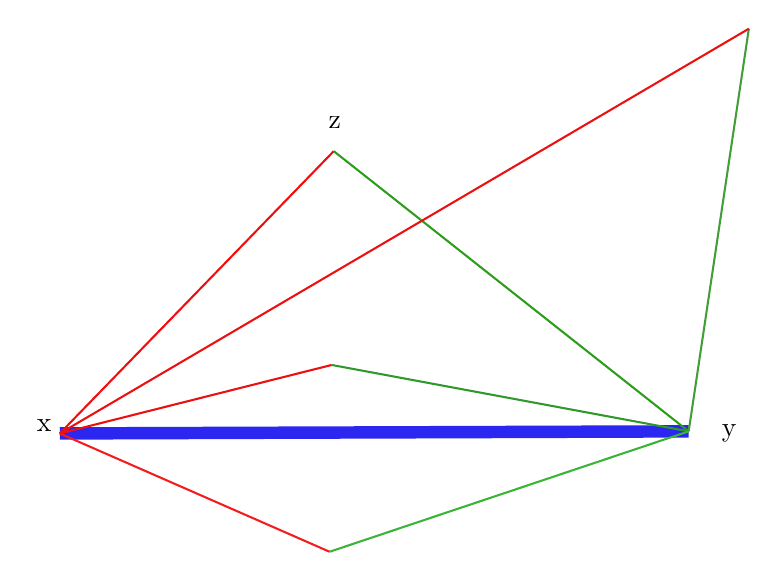
\begin{tikzpicture}[x=0.75pt,y=0.75pt,yscale=-1,xscale=1]
%uncomment if require: \path (0,300); %set diagram left start at 0, and has height of 300

%Straight Lines [id:da6847309088840179] 
\draw [color={rgb, 255:red, 44; green, 38; blue, 241 }  ,draw opacity=1 ][line width=4.5]    (69.5,214) -- (372.5,213) ;


%Straight Lines [id:da46426148005512835] 
\draw [color={rgb, 255:red, 241; green, 13; blue, 13 }  ,draw opacity=1 ]   (201.5,78) -- (69.5,214) ;


%Straight Lines [id:da2906024541588399] 
\draw [color={rgb, 255:red, 46; green, 156; blue, 29 }  ,draw opacity=1 ]   (201.5,78) -- (372.5,213) ;


%Straight Lines [id:da6028165286195768] 
\draw [color={rgb, 255:red, 236; green, 15; blue, 15 }  ,draw opacity=1 ]   (69.5,214) -- (200.5,181) ;


%Straight Lines [id:da6610711832317098] 
\draw [color={rgb, 255:red, 47; green, 153; blue, 44 }  ,draw opacity=1 ]   (200.5,181) -- (372.5,213) ;


%Straight Lines [id:da7902181564457826] 
\draw [color={rgb, 255:red, 243; green, 29; blue, 29 }  ,draw opacity=1 ]   (69.5,214) -- (199.5,271) ;


%Straight Lines [id:da8016282193076851] 
\draw [color={rgb, 255:red, 58; green, 179; blue, 54 }  ,draw opacity=1 ]   (372.5,213) -- (199.5,271) ;


%Straight Lines [id:da6023664239656019] 
\draw [color={rgb, 255:red, 67; green, 158; blue, 57 }  ,draw opacity=1 ]   (401.5,19) -- (372.5,213) ;


%Straight Lines [id:da5175708881441581] 
\draw [color={rgb, 255:red, 235; green, 17; blue, 17 }  ,draw opacity=1 ]   (401.5,19) -- (69.5,214) ;



% Text Node
\draw (62,210) node  [align=left] {x};
% Text Node
\draw (392,214) node  [align=left] {y};
% Text Node
\draw (202,64) node  [align=left] {z};


\end{tikzpicture}
\label{desitri}
\end{center}




Na figura \ref{desitri} a desigualdade triangular é clara. Em qualquer um dos triângulos, a soma do comprimento das arestas vermelha e verde é sempre menor que a azul. Existem variadas métricas, apresento aqui alguns exemplos:

\begin{itemize}
    \item \textbf{Métrica Euclidiana:} $d(x,y) = \sqrt{\sum_{i=1}^k (x_i - y_i)^2}$. Esta é a noção usual de distância que temos. Com esta métrica, o menor trajeto entre dois pontos sempre é uma reta. Observe que em uma dimensão a métrica euclidiana é simplesmente $x-y$. Em duas é o tamanho da hipotenusa do triângulo retângulo inscrito nos dois pontos. Em três é o tamanho da diagonal do cubo inscrito nos pontos e por aí vai.
    \item \textbf{Métrica Discreta:} $d(x,y) = \mathbb{1}(x \neq y)$. Uma noção um pouco curiosa de distância em que se dois elementos são diferentes dizemos que distam uma unidade. 
    \item \textbf{Métrica "Taxista":} $d(x,y) = \sqrt{\sum_{i=1}^d (x_i - y_i)}$
\end{itemize}



\subsection{Espaços Métricos}

\begin{defi}
Um \textbf{Espaço Métrico} é uma dupla de um conjunto $X$ e uma métrica $d$. Nos referimos ao espaço munido deste ambiente e dessa noção de distância como $(X,d)$.
\end{defi}

Esse conceito é mais fino e amplo do que parece à primeira vista. Estamos falando de conjuntos, então meras coleções de elementos, e de métricas, maneiras de medir distâncias. Digamos que estamos no plano cartesiano. Um conjunto qualquer prontamente se torna um espaço métrico ao munirmos ele de uma métrica - Euclidiana, discreta ou que for - e agora ganhamos espaço de manobra para garantir que certos fenômenos ocorram nele.

O poder de pensar em termos de Espaços Métricos com tanta generalidade é que conseguimos ver com mais clareza o que há de comum entre o plano cartesiano e a superfície arredondada da terra - e como espaços diferentes podem por vezes pedir métricas diferentes para responderem problemas de ordem mais prática. Conceber distância como a reta que liga dois pontos faz muito sentido no plano cartesiano ou no $\mathbb{R}^k$, mas nem tanto ao falar da superfície da terra, em que normalmente modelamos a distância entre dois pontos como o menor arco na superfície que ligue-os. 




\subsection{Sequências e Limites}


\begin{defi}
Uma \textbf{sequência} $x:\mathbb{N} \to \mathbb{R}^k$ é uma função que mapeia os naturais em elementos de algum conjunto. Podemos, alternativamente, entender uma sequência como um conjunto $\{x_n\} = \{ x_n \in \mathbb{R}^k \,\, | \,\, n \in \mathbb{N}\}$. Dizemos que uma sequência tem \textbf{limite} em $L$ - alternativamente que $L$ é limite de $x_n$ ou que $x_n$ \textbf{converge} a $L$ - se $\forall \,\, \epsilon > 0 \,\, \exists \,\, n' \in \mathbb{N} \,\, | \,\, n > n' \implies d(x_n, L) < \epsilon$. Notamos $\lim_{n \to \infty} x_n = L$
\end{defi}

Sequências são apenas conjuntos de elementos com um processo definidor. Imagine por exemplo a sequência contida na reta real $x_n = \frac{1}{n}$, ou uma prima não-muito-distante contida no $\mathbb{R}^2$, $y_n = (\frac{1}{n}, \frac{10}{n})$. Observe que $\lim x_n = 0$ e que $\lim y_n = (0,0)$. Podemos construir uma infinidade de outros exemplos, seguem alguns - todos com a métrica euclidiana em mente.

\begin{itemize}
    \item $x_n = (1 + \frac{1}{n})$ \implies 
    $\lim x_n = 1$ 
    \item $x_n = (1, 2n, \frac{79}{n})$ \implies
    $\lim x_n = (1, \infty, 0)$
    \item $x_n = \sin{n}$ \implies
    $\nexists \lim x_n$
    \item $x_n = (1+\frac{1}{n})^n$ \implies $\lim x_n = e$
    \item $x_n = (-\frac{4n^2}{3n}, n, \pi)$ \implies $\lim x_n = (-\infty, \infty, \pi)$
    \item $x_n = 2$ \implies $\lim x_n = 2$
\end{itemize}


Aos nos referir a números arbitrariamente pequenos como $\epsilon > 0$ estamos tão somente dizendo que não importa o quão arbitrariamente próximo de um ponto limite quer-se chegar, se uma sequência converge a este limite, existe algum índice natural tal que a sequência está à uma distância menor que $\epsilon$ deste limite. Observe que não importando qual natural seja escolhido, a rigor, $\frac{1}{n}$ jamais será de fato igual a zero e sim à grandezas arbitrariamente pequenas. No entanto, dada uma distância arbitrária do zero, sempre podemos atingi-la com este sequência que tenha limite em zero ao escolher um $n$ suficientemente grande. Esta é a noção de limite.

Talvez agora comece a fazer um pouco mais de sentido a escolha deliberada de falar com generalidade de distâncias. $x_n = 1/n$ por exemplo tem limite em $0$ na métrica euclidiana, mas na discreta não.

\subsection{Sequências de Cauchy}

Temos agora um pequeno problema teórico em mãos. A depender da métrica, algumas sequências cujos termos se aproximam arbitrariamente de certos pontos podem ou não ter limites. Como lidamos com isso? Abriremos mão da noção de limite e focaremos no comportamento em si: termos de uma sequência que estão cada vez menos distantes entre si.

\begin{defi}
Uma sequência é \textbf{de Cauchy} se $\forall \,\, \epsilon > 0 \,\, \exists \,\, n \in \mathbb{N} \,\, | \,\, a,b > n \implies d(x_a,x_b) < \epsilon$.
\end{defi}

Uma sequência de Cauchy apresenta essa propriedade de que para qualquer distância arbitrária de $0$ que se escolha, existe algum ponto a partir do qual todos os termos da sequência distam no máximo essa distância arbitrária, por menor que seja. Uma sequência de Cauchy é, no português mais direto, uma em que os termos subsequentes estão sempre cada vez mais próximos.

Essa noção pode ser difícil de diferenciar de uma sequência que tem limite em algum ponto então façamos um pequeno exercício mental. Imagine que estamos no espaço métrico $(\mathbb{Q}, d)$. Imagine agora a seguinte sequência:

$$a_1 = 3$$
$$a_2 = 3,1$$
$$a_3 = 3,14$$
$$a_4 = 3,141$$
$$a_5 = 3,1415$$
$$a_6 = 3,14159$$
$$...$$
$$a_{30} = 3,1415926535 8979323846 2643383279$$
$$...$$

Eu espero que seja claro ao leitor que essa sequência $a_n$ é de Cauchy. O que não pode parecer claro a princípio é que, apesar disso, não existe limite para essa sequência. Isto porque ela se aproxima arbitrariamente de $\pi$ e estamos no espaço métrico $(\mathbb{Q}, d)$. Esta sequência está indo \textbf{para fora} do espaço -  porque $\pi$ é um número irracional - ainda que seja de Cauchy e tenha termos cada vez mais próximos uns dos outros. 

\subsection{Espaços Métricos Completos}

Note que se descrevermos uma sequência de Cauchy em um espaço que esteja se aproximando de um elemento desse mesmo espaço, ela necessariamente converge, temos um limite. Será então que existem espaços em que \textbf{toda} sequência de Cauchy converge? Já sabemos que isso claramente não procede para espaços $(\mathbb{Q}, d)$, qualquer que seja a métrica.

Voltemos ao exemplo da sequência $a_n$ que se aproximava de $\pi$. Se fizermos uma operação de "colar" esse buraco faltando nos reais, a história muda. Imagine o conjunto $A = \mathbb{Q} \bigcup \{\pi\}$. Se estivermos no espaço $(A,d)$ então $\exists \lim a_n$ e mais ainda, $\lim a_n = \pi$. Isso nos deixa agora com outra infinidade de sequências que são de Cauchy e não convergem no espaço $(A,d)$ porque se aproximam arbitrariamente de números irracionais como $e$ e $\sqrt{2}$. Repetindo a operação de colar os irracionais até que tenhamos colado todos faz com que $A = \mathbb{Q} \bigcup \mathbb{I}$. 

Perceba que a união dos racionais com os irracionais dá o conjunto dos números reais e que por construção qualquer sequência de Cauchy em um espaço $(\mathbb{Q} \bigcup \mathbb{I}, d)$ converge. É impossível construir uma sequência de Cauchy de números reais que não tenha como limite outro número real. Em um espaço métrico construído com números reais, \textbf{toda} sequência de Cauchy converge. Este fato é notável e merece uma conceitualização própria.

\begin{defi}
Um espaço métrico $(X,d)$ é \textbf{completo} se nele toda sequência de Cauchy converge.
\end{defi}

Os Reais caracterizam um espaço métrico completo. Ao contrário do que ocorre nos Irracionais e nos Racionais, ambos permeados de "buracos". Completude é uma propriedade muito interessante de espaços métricos e veremos mais à frente que ela é central para a validade de alguns teoremas extremamente úteis como o do Ponto Fixo de Banach. 

Recapitulando, começamos esta seção falando de métricas. Apenas formalizamos nossa intuição sobre o que significam distâncias. A partir daí construímos um novo conceito, o de sequências e vimos que sequências são maneiras de nos aproximarmos de números de maneiras arbitrárias. Vimos depois que a depender de qual conjunto usamos para construir nossos espaços métricos, se aproximar arbitrariamente de um ponto não quer dizer convergir a ele. Por isso refinamos nosso conceito de sequência e conhecemos as sequências de Cauchy. Logo uma pergunta absolutamente natural emergiu. Queríamos saber se existem espaços em que ter um limite e ser uma sequência de Cauchy são sinônimos. Por serem "especiais" nesse sentido, demos a eles um nome específico: espaços métricos completos. E assim o são por não terem os "buracos" que racionais e irracionais têm.

Agora voltamos nossas miras para a topologia elementar ponto-a-conjunto, onde estudaremos as propriedades mais gerais de conjuntos e de espaços. 

\section{Topologia Ponto-a-Conjunto Elementar}
\label{segunda}




\subsection{Interioridade e Abertura}
\subsection{Vizinhanças e Bolas}
\subsection{Aderência e Proximidade}
\subsection{Limitação e Compacidade}
\subsection{Teorema de Bolzano-Weierstrass}


\section{Funções, Continuidade e Pontos Fixos}
\label{terceira}
\subsection{Mapa, função, transformação, campo ou correspondência?}
\subsection{Compacidade e Continuidade}
\subsection{Homeomorfismos, Retrações, Contrações e outras formas de deformar espaços}
\subsection{Um brevíssimo passeio pelos Teoremas de Ponto Fixo}
\subsubsection{Os Teoremas de Brouwer e Kakutani: Deformando Conjuntos Convexos}
\subsubsection{O Teorema do Ponto Fixo de Banach: Contraindo Espaços Completos}



\section{Mapeando Espaços de Funções}
\label{quarta}
\subsection{Espaços de Funções}
\subsection{Equações Diferenciais como Mapas do Espaço de Funções}
\subsection{Equações em Diferenças e Mapas Iterados}


\chapter{Processos Estocásticos}

Aqui faço uma exposição breve, autocontida e razoavelmente formal do objeto central deste estudo.


\begin{defi}

Um \textbf{Processo Estocástico n-dimensional} é uma sequência  $\{X_t\}_{t \in T} \subset \Omega \subseteq \mathbb{R}^n$ onde $X_t$ é uma variável aleatória e o conjunto $T = \{1,2,...,t\}$ indexa a passagem do tempo.  
\end{defi}

Confrontados com dados do mundo real, observamos apenas \textbf{uma} realização particular do processo qualquer que comande o fenômeno estudado. Logo, ao descrever a realização do processo como uma sequência, ela necessariamente caracterizará um subconjunto próprio do espaço amostral $\Omega$. 

\section{Processos Autoregressivos}

%-------------------------------------------------------------------
% O que faremos abaixo é incluir uma imagem (formato JPG, mas 
% poderia ser outro formato) no pdf. O argumento width=\textwidth 
% ajusta a largura da imagem a largura da página
%-------------------------------------------------------------------

%\begin{figure}[h]
%	\includegraphics[width=\textwidth%]{imagens/blocof.jpg}
%	\caption{O Bloco F}
%	\label{fig:blocof} % Aqui %'nomeamos' o gráfico
%\end{figure}

%-------------------------------------------------------------------
% mais lipsum...
%-------------------------------------------------------------------
